\documentclass[12pt,twoside]{report}
\usepackage{lmodern}
\usepackage{setspace}
\setstretch{1.5}
\usepackage{amssymb,amsmath}
\usepackage{ifxetex,ifluatex}
%\usepackage{fixltx2e} % provides \textsubscript
\ifnum 0\ifxetex 1\fi\ifluatex 1\fi=0 % if pdftex
  \usepackage[T1]{fontenc}
  \usepackage[utf8]{inputenc}
\else % if luatex or xelatex
  \ifxetex
    \usepackage{mathspec}
  \else
    \usepackage{fontspec}
  \fi
  \defaultfontfeatures{Ligatures=TeX,Scale=MatchLowercase}
\fi
% use upquote if available, for straight quotes in verbatim environments
\IfFileExists{upquote.sty}{\usepackage{upquote}}{}
% use microtype if available
\IfFileExists{microtype.sty}{%
\usepackage{microtype}
\UseMicrotypeSet[protrusion]{basicmath} % disable protrusion for tt fonts
}{}
\usepackage[left=3cm, right=3cm, top=2.5cm, bottom=2.5cm]{geometry}
\usepackage{hyperref}
\PassOptionsToPackage{usenames,dvipsnames}{color} % color is loaded by hyperref
\hypersetup{unicode=true,
            pdftitle={From Panopticon to Palantír: Algorithmic Governance in the Post-Disciplinary Societies},
            pdfauthor={Bachelorarbeit; Universität Wien; LV-Leiter: Dr.~Matthias Flatscher \textbar{} LV: 2018W 210090-1 BAK18},
            colorlinks=true,
            linkcolor=Maroon,
            citecolor=Blue,
            urlcolor=blue,
            breaklinks=true}
\urlstyle{same}  % don't use monospace font for urls
\usepackage{longtable,booktabs}
\usepackage{graphicx,grffile}
\makeatletter
\def\maxwidth{\ifdim\Gin@nat@width>\linewidth\linewidth\else\Gin@nat@width\fi}
\def\maxheight{\ifdim\Gin@nat@height>\textheight\textheight\else\Gin@nat@height\fi}
\makeatother
% Scale images if necessary, so that they will not overflow the page
% margins by default, and it is still possible to overwrite the defaults
% using explicit options in \includegraphics[width, height, ...]{}
\setkeys{Gin}{width=\maxwidth,height=\maxheight,keepaspectratio}
\IfFileExists{parskip.sty}{%
\usepackage{parskip}
}{% else
\setlength{\parindent}{0pt}
\setlength{\parskip}{6pt plus 2pt minus 1pt}
}
\setlength{\emergencystretch}{3em}  % prevent overfull lines
\providecommand{\tightlist}{%
  \setlength{\itemsep}{0pt}\setlength{\parskip}{0pt}}
\setcounter{secnumdepth}{5}
% Redefines (sub)paragraphs to behave more like sections
\ifx\paragraph\undefined\else
\let\oldparagraph\paragraph
\renewcommand{\paragraph}[1]{\oldparagraph{#1}\mbox{}}
\fi
\ifx\subparagraph\undefined\else
\let\oldsubparagraph\subparagraph
\renewcommand{\subparagraph}[1]{\oldsubparagraph{#1}\mbox{}}
\fi

%%% Use protect on footnotes to avoid problems with footnotes in titles
\let\rmarkdownfootnote\footnote%
\def\footnote{\protect\rmarkdownfootnote}

%%% Change title format to be more compact
\usepackage{titling}

% Create subtitle command for use in maketitle
\newcommand{\subtitle}[1]{
  \posttitle{
    \begin{center}\large#1\end{center}
    }
}

\setlength{\droptitle}{-2em}

  \title{From Panopticon to Palantír: Algorithmic Governance in the Post-Disciplinary Societies}
    \pretitle{\vspace{\droptitle}\centering\huge}
  \posttitle{\par}
  \subtitle{Utku Bilen Demir \textbar{} 0848242}
  \author{Bachelorarbeit \\ Universität Wien \\ LV-Leiter: Dr.~Matthias Flatscher \textbar{} LV: 2018W 210090-1 BAK18}
    \preauthor{\centering\large\emph}
  \postauthor{\par}
      \predate{\centering\large\emph}
  \postdate{\par}
    \date{25.02.2019}

\usepackage{booktabs}
\usepackage{fontspec}
\usepackage{dcolumn}
\usepackage{longtable}

\usepackage{booktabs}
\usepackage{array} 
\usepackage{multirow}
\usepackage{wrapfig}
\usepackage{float}
\usepackage{colortbl}
\usepackage{pdflscape}
\usepackage{tabu}
\usepackage{threeparttable}
\usepackage{threeparttablex}
\usepackage[normalem]{ulem}
\usepackage{makecell}
\usepackage{xcolor}
\usepackage{pdfpages}

\pagestyle{plain}
\raggedbottom 

\setmainfont{Palatino Linotype}




\let\oldhref\href
\renewcommand{\href}[2]{#2\footnote{\url{#1}}}

\begin{document}
\maketitle
\begin{abstract}
Algorithmic processes that operate on the massive data traffic the participatory web culture \emph{WEB 2.0} brought personalize and shape the digital reality of the individuals by controlling the information flow. This paper aims to analyze the contemporary algorithmic governance on digital networks through a Foucauldian perspective to analyze its mechanism in the context of biopolitics and draw connections to different arts of governances.
\end{abstract}

{
\hypersetup{linkcolor=black}
\setcounter{tocdepth}{5}
\tableofcontents
}
\listoftables
\listoffigures
\newpage

\pagebreak
\hspace{2pt}
\vfill

\emph{Ich erkläre hiermit, dass ich die vorliegende schriftliche Arbeit selbstständig verfertigt habe und dass die verwendete Literatur bzw. die verwendeten Quellen von mir korrekt und in nachprüfbarer Weise zitiert worden sind. Mir ist bewusst, dass ich bei einem Verstoß gegen diese Regeln mit Konsequenzen zu rechnen habe.}
\vfill
\hspace{2pt}
\pagebreak

\hypertarget{introduction}{%
\chapter{Introduction}\label{introduction}}

\begin{center}\rule{0.5\linewidth}{\linethickness}\end{center}

The notion of surveillance has changed rapidly with the emergence of the digital age. The automated collection of vast amount of data, along with the ramification of the participatory internet culture \emph{Web 2.0} (O'reilly \protect\hyperlink{ref-Oreilly2009}{2009}), drastically changed the level of \emph{visibility} of the \emph{digital subjects} (Krasmann \protect\hyperlink{ref-Krasmann2017}{2017}). As the complexity of the data increased rapidly in the last decades, the use of the algorithmic processes to automate specific tasks became a fundamental process on the web. Once naive, step-by-step instructions that solved simple computational problems evolved into complex systems that govern the digital realm. Algorithmic systems today index the content on the internet, categorize the data, profile the users, make anticipations about the future behavior, and shape the digital reality of the individuals by controlling the information flow. As the decision-making abilities of the algorithmic systems increase by the day with the new developments that enable algorithms to function with less supervision, the extent and the contemporary characteristics of the algorithmic governance arouses questions about the power of the governance algorithmic systems deploy. A comprehensive analysis to understand contemporary algorithmic governance scheme is not an easy task; the complexity of their structure, the opacity of the code, the need for an interdisciplinary approach make it a challenge to open the \emph{black box} of algorithmic operations. The inspiration of this paper emerges from the pursuit to analyze the art of governance that algorithmic processes seemingly deploy through a Foucauldian perspective to gain insight in the mechanics of our digital reality and discuss the operation in the context of biopolitics.

Michel Foucault has been a central name in the study of power. Following Foucault's journey on the analysis of biopower Chapter \ref{theory} starts with the discussion of the Foucault's work \emph{Discipline and Punish} (\protect\hyperlink{ref-Foucault1995}{1995}). The emergence of a power structure that concentrates explicitly on the conduct of its subjects and uses the means of surveillance as a technology to shape the subjectivity of the individuals constitutes the foundation of what Foucault calls the \emph{disciplinary society} (Foucault \protect\hyperlink{ref-Foucault1995}{1995}, 209). Foucault explains the role of surveillance in the disciplinary power with the metaphor of Jeremy Bentham (\protect\hyperlink{ref-Bentham1843}{1843})'s theoretical prison structure \emph{Panopticon} which increases the efficiency of surveillance by exposing the individuals to constant visibility and concealing the observer. While the subjects never know if and when they are surveilled, under the pressure of the possibility disciplinary power produces docile bodies, the training into a specific subjectivity becomes a self-praxis. The concentration of the power structure over bodies, pursuit of production of docility marks the beginning of the \emph{biopolitics}. In this regard, this paper aims to answer the question:

\begin{quote}
\emph{RQ: How should the underlying mechanism of the contemporary algorithmic governance structure be understood in the context of biopolitics?}
\end{quote}

The research question intents to ground a broad discussion about the significance and role of the algorithms in the contemporary mechanism of biopolitics; however, Foucault analyzes biopower and -politics concepts in the context of different arts of governances first in his later published works. In order to form an introduction to Foucault's biopower and -politics concepts, after the analysis of the disciplinary power, Chapter \ref{theory} mainly deals with Foucault's lectures in Collège de France which were published under the name \emph{The Birth of Biopolitics} (\protect\hyperlink{ref-Foucault2008}{2008}); as complementary literature Thomas Lemke (\protect\hyperlink{ref-Lemke2001}{2001})'s reading of Foucault also constitutes an important part of the discussion. In Birth of Biopolitics, Foucault analyzes exclusively different biopolitical structures in liberal and neo-liberal governmentalities\footnote{Foucault creates the word governmentality by linking the words governing (\emph{gouverner}) and mentality (\emph{mentalité}) to name the art of governing (Lemke \protect\hyperlink{ref-Lemke2001}{2001}, 191).}. Foucault's refusal to see neo-liberal art of governance as a follower of its liberal counterpart creates the opportunity to test the algorithmic governance with two distinct types of governmentalities. As Foucault states, the unique approach of the neo-liberal thought to the rationality of the subject, human behavior and social environment with the principles of economic analysis allows me to build the hypothesis on the possible similarities between neo-liberal governmentality and algorithmic governance as follows:

\begin{quote}
\emph{H: Algorithmic governance of the information on the web transforms surveillance into a non-disciplinary normalization exercise in alignment with Michel Foucault's definition of the characteristics of neo-liberal governmentality.}
\end{quote}

After Chapter \ref{theory} follows the lines of the methodology of literary analysis; Chapter \ref{alg} firstly deals with the definition of algorithms as well as the history of digital surveillance and the contemporary mechanics of the digital networks by citing multiple works on the issue. Thereafter, following the steps of an algorithmic selection (Just and Latzer \protect\hyperlink{ref-Just2017}{2017}), I aim to define the inner mechanism of the algorithmic governance from data collection to the construction of the personalized information flow. In the same process, specific features about the algorithmic processes like the problem of opacity and developments like machine learning approach also construct further discussion. In this process, I explicitly emphasize the works of John Cheney-Lippold((\protect\hyperlink{ref-Cheney2011}{2011})\&(\protect\hyperlink{ref-Cheney2017}{2017})) as well as Antoinette Rouvroy, Berns, and Libbrecht (\protect\hyperlink{ref-Rouvroy2013}{2013}) and Martjin Van Otterlo (\protect\hyperlink{ref-Otterlo2013}{2013}). The technical analysis of the algorithmic reality construction process (Just and Latzer \protect\hyperlink{ref-Just2017}{2017}) as well as the short history of the big data and participatory web culture in Chapter \ref{alg} enables the interpretation of the algorithmic governance in the context of Foucault's theory in Chapter \ref{hob}. While I draw connections between specific aspects of the theoretical basis of neo-liberal governmentality to the algorithmic governance, I also mention Gilles Deleuze (\protect\hyperlink{ref-Deleuze1992}{1992})'s contribution to the topic with his short essay \emph{Postscript on the Societies of Control} as a guideline to name specific concepts.

\hypertarget{theory}{%
\chapter{\texorpdfstring{The Forge of Subjectivity: \emph{Surveillance and Governmentality in Michel Foucault's Political Theory}}{The Forge of Subjectivity: Surveillance and Governmentality in Michel Foucault's Political Theory}}\label{theory}}

\begin{center}\rule{0.5\linewidth}{\linethickness}\end{center}

Michel Foucault is a central name in the study of power; his works have widely been an inspiration for the studies on the mechanics of political structure and modern society. This chapter follows Foucault's perspective on the modern art of governance(s) in two parts; starting first with Foucault's central work \emph{Discipline and Punish} (\protect\hyperlink{ref-Foucault1995}{1995}) and following mainly his later published work \emph{Birth of Biopolitics} (\protect\hyperlink{ref-Foucault2008}{2008}) on the second part.

\hypertarget{discipline}{%
\section{Discipline}\label{discipline}}

\begin{quote}
Power is everywhere; not because it embraces everything, but because it comes from everywhere.

--- (Foucault \protect\hyperlink{ref-Foucault1978}{1978}, 93)
\end{quote}

Michel Foucault's \emph{Discipline and Punish} begins with the famous example of the horrifying punishment \emph{Robert-François Damiens}, the perpetrator of an attempted regicide, has gone through. The brutality and public spectacle of the punishment were parts of a mechanism to restore and reaffirm the power of the sovereign (Gane \protect\hyperlink{ref-Gane2012}{2012}, 614). The penal system, however, has gone through a series of rapid transformations in the following period; the public spectacle, as well as the torture, gradually vanished in Europe. The new punitive structure replaced the spectacle of punishment with a new model that worked through \emph{correction and normalization} of the body (cf. Gane \protect\hyperlink{ref-Gane2012}{2012}, 614). The theory of sovereignty was mostly bound to the land and the products extracted from it. However, with the emergence of the capitalist mode of production the human body, its labor and its doing, became a point of interest for power. The overarching structure of the sovereign power was unable to achieve the micro-management of the bodies; it led eventually to the birth of a non-sovereign type of power, which Foucault calls as one of bourgeois society's great inventions, the \emph{disciplinary power} (cf. Foucault \protect\hyperlink{ref-Foucault2003}{2003}, 35--36). Foucault describes disciplinary power with its new type of political investment in the human body:

\begin{quote}
{[}\ldots{}{]} its{[}body's{]} constitution as labour power is possible only if it is caught up in a system of subjection {[}\ldots{}{]} ; the body becomes a useful force only if it is both a productive body and a subjected body. This subjection is not only obtained by the instruments of violence or ideology; it can also be direct, physical, pitting force against force, bearing on material elements, and yet without involving violence; it may be calculated, organized, technically thought out; it may be subtle, make use neither of weapons nor of terror and yet remain of a physical order.

--- (Foucault \protect\hyperlink{ref-Foucault1995}{1995}, 25--26)
\end{quote}

The strive for a certain kind of \emph{knowledge} to obtain the mentioned subjugation marks in Foucault's perspective the fundamental nature of \emph{disciplinary society} (Foucault \protect\hyperlink{ref-Foucault1995}{1995}, 209). This new type of \emph{political technology of the body} (ibid., 26) is not a specific apparatus or institution; moreover, if we look at this power structure through Foucault's perspective, there is nothing monolithic about it. It is not possessed by someone; it is not just the property of a privileged class, not acquired or preserved; it is constantly active and resides in the diffuse techniques, tactics, societal functions in a network. In this sense, it is also manifested and extended by its subjects. Therefore, one needs to analyze the \emph{microphysics of power} (Foucault \protect\hyperlink{ref-Foucault1995}{1995}, 26--27), its manifestations in the subtle relationships and mechanisms, not to find someone who holds or exercises it but in order to grasp the strategy all those small components reveal inductively, once they are brought together.

\hypertarget{knowledgepower}{%
\subsection{Knowledge/Power}\label{knowledgepower}}

The analysis of \emph{the power over bodies} is the starting point of Foucault's concept of \emph{bio-politics}. As the altering of human conduct, disciplination of the bodies become the main drive of the power, the role of the knowledge in this process also ramifies. The production of knowledge develops necessary mediums to shape the conduct in the chosen \emph{cast}. Foucault gives the example of the \emph{invention} of a soldier. The \emph{correct training} that obtained throgh the knowledge made it possible to turn a peasant into a soldier (Foucault \protect\hyperlink{ref-Foucault1995}{1995}, 135). The disciplinary power operates in the society in the same manner by shaping the human \emph{soul}. Foucault's concept of soul, however, differs greatly from the common use of the word. The soul is according to Foucault is an element which has been shaped by the effects of the operating power structure through the knowledge over the subject (cf. Foucault \protect\hyperlink{ref-Foucault1995}{1995}, 29). The soul represents the subjectivity, and it is the societal relations that forge the subjectivity in its journey. The success of the disciplinary power emerges from the possibility of the production of a certain kind of subjectivity, by grasping the body through the soul. In this regard, science also has a great role in this process; Foucault's approach implicates that it is not about discovering the truth but producing certain truths; certain truths that expose its subjects to the power by making them knowable and accessible (cf. Krasmann \protect\hyperlink{ref-Krasmann2017}{2017}, 11). Foucault discusses the relationship between power and knowledge as follows:

\begin{quote}
We should admit rather that power produces knowledge (and not simply by encouraging it because it serves power or by applying it because it is useful); that power and knowledge directly imply one another; that there is no power relation without the correlative constitution of a field of knowledge, nor any knowledge that does not presuppose and constitute at the same time power relations.

--- (Foucault \protect\hyperlink{ref-Foucault1995}{1995}, 27)
\end{quote}

The production of the knowledge on bodies, however, not just an external process applied by the study of science; knowledge production is, firstly, a discourse circularly produces itself in the societal relations by producing a specific understanding of rationality; secondly, the knowledge about bodies also produced through observation (cf. Foucault \protect\hyperlink{ref-Foucault1995}{1995}, 249). Surveillance is, therefore, a central notion in the disciplinary society.

\hypertarget{panopticism}{%
\subsection{Panopticism}\label{panopticism}}

\begin{quote}
Our society is one not of spectacle, but of surveillance; under the surface of images, one invests bodies in depth; behind the great abstraction of exchange, there continues the meticulous, concrete training of useful forces; {[}\ldots{}{]} it is not that the beautiful totality of the individual is amputated, repressed, altered by our social order, it is rather that the individual is carefully fabricated in it, according to a whole technique of forces and bodies.

--- (Foucault \protect\hyperlink{ref-Foucault1995}{1995}, 217)
\end{quote}

The most distinctive feature of the disciplinary power structure is the effective use of the means of surveillance. It is what makes disciplinary power in comparison to the reign of a sovereign more continuous and encircling (cf. Foucault \protect\hyperlink{ref-Foucault1980}{1980}, 103--4). The superiority of the disciplinary surveillance methods lies not the expenditure invested in it, but in the machinery, the specific power structure developed to make observance limitless and omnipresent in the society (Foucault \protect\hyperlink{ref-Foucault1995}{1995}, 214). Foucault takes Jeremy Bentham's concept of Panopticon(\protect\hyperlink{ref-Bentham1843}{1843}) as a symbolic representation of that mechanism.

Bentham's Panopticon is a theoretical prison concept where all the cells are lined on the perimeter in an annular building, and there stands a watchtower at the center. The watchtower is able to observe all of the cells, but the inner room of the tower is, be it with blinds or one-way mirrors, obscured. The inmates are always observable from the watchtower, but they are not able to see whether someone is standing in the tower (cf. Foucault \protect\hyperlink{ref-Foucault1995}{1995}, 200). Panopticon's effectiveness relies on a few specific features in this regard. Firstly, it allows fewer people to exercise surveillance while increasing the number of those whom it is exercised, effectiveness and continuously increase while the expenditure falls. Secondly; on the one hand, it generates anonymity for the ones who exercise the surveillance and on the other hand makes it possible for anyone to operate the machinery (cf. Bentham \protect\hyperlink{ref-Bentham1843}{1843}, 45--66). Thirdly it leaves the inmates in a \emph{field of visibility}, under a constant pressure of being observed that normalizes their conduct (Foucault \protect\hyperlink{ref-Foucault1995}{1995}, 202).

Panopticon's machinery became an underlying function in the disciplinary society. It is not that the subject is under constant surveillance in the disciplinary society, rather than, it is the pressure of being visible. It is the transformation of the power to be more effective and economical, instead of being an external force the power becomes a part of the subject, the eye of the disciplinary power will be inverted in the mind (Gehring \protect\hyperlink{ref-Gehring2017}{2017}). Being exposed to \emph{a state of conscious and permanent visibility} is the fictitious relation Foucault sees what makes the subject the principle of her own subjection (cf. Foucault \protect\hyperlink{ref-Foucault1995}{1995}, 202--3). The \emph{modern state} is, therefore, not an overarching compound above individuals but, on the contrary, it is a sophisticated structure which bounds the integration of the individual into its realm to one condition that her individuality will be shaped in a new form and submitted to a set of specific patterns (Foucault \protect\hyperlink{ref-Foucault1982}{1982}, 783), Panopticism represents, in this sense, a \emph{new political anatomy} (Foucault \protect\hyperlink{ref-Foucault1995}{1995}, 208).

\hypertarget{governmentalities-and-the-subjectivity}{%
\section{Governmentalities and the subjectivity}\label{governmentalities-and-the-subjectivity}}

Panopticon-metaphor have been a central notion in the surveillance-related studies, however, although Foucault makes connections between panoptic surveillance and the liberal art of governance, the political application of the panoptic structure, its role in the art of governance as well as the transformations in the mechanics of discipline is not addressed in Discipline and Punish (cf. Gane \protect\hyperlink{ref-Gane2012}{2012}, 617). Foucault analyzes different arts of governance in liberalism and neo-liberalism, along with the subjectivities both governance art produces, especially in his later published Lectures in Collège de France under the name \emph{The Birth of Biopolitics}.

\hypertarget{neo-liberal-governmentality}{%
\subsection{Neo-liberal Governmentality}\label{neo-liberal-governmentality}}

Foucault's analysis of neo-liberalism starts with his refusal of three misleading hitherto definitions. First, that neo-liberalism nothing more than the reactivation of old economic theories; second, that it is just a way to establish strict market relations in society; and third, that neo-liberalism is no more than a cover for a generalized administrative intervention by the state (Foucault \protect\hyperlink{ref-Foucault2008}{2008}, 130). The misleading part of those attempts for a definition is their underlying claim that neo-liberalism is just an ordinary follower, an accelerated sequel of classical liberalism, \emph{a worse version of the same thing} (cf.~ibid.). Those three approaches firstly prevent an analysis about an individual neo-liberal \emph{Weltanschauung} and secondly carry the assumption that the machinery neo-liberal governmentality use have to be the upgraded forms of those from the liberal art of government.

The uniqueness of neo-liberalism lies in its specific art of governmentality according to Foucault. Instead of freeing space for the market by reforming the governmental structure as in the classical liberalism, neo-liberalism tries to install formal market principles of the market economy as the general art of government (Foucault \protect\hyperlink{ref-Foucault2008}{2008}, 131). Foucault emphasizes the difference between classical liberalism and those neo-liberalist school of thoughts with their approach to the notion of \emph{laissez-faire}. While in classical liberalism a well-functioning market is a natural follower of the pursued laissez-faire setting, in neo-liberal governmentality the notion of governing will be shaped directly through market principles, \emph{one will govern for the market rather than because of the market} (Foucault \protect\hyperlink{ref-Foucault2008}{2008}, 121).

Something to note here is, as Thomas Lemke (\protect\hyperlink{ref-Lemke2001}{2001}) emphasizes in his reading, Foucault's use of the term \emph{government}. Foucault uses this term in its earlier meaning in a broader sense as he mentions as following:

\begin{quote}
This word must be allowed the very broad meaning which it had in the sixteenth century. ``Government'' did not refer only to political structures or to the management of states; rather, it designated the way in which the conduct of individuals or of groups might be directed: the government of children, of souls, of communities, of families, of the sick. It did not only cover the legitimately constituted forms of political or economic subjection but also modes of action, more or less considered or calculated, which were destined to act upon the possibilities of action of other people. To govern, in this sense, is to structure the possible field of action of others.

--- (Foucault \protect\hyperlink{ref-Foucault1982}{1982}, 789--90)
\end{quote}

Thereby, as Foucault mentions the distinct features of the neo-liberal governmentality, he finds its strongest implications in the technologies of power this particular art of government possess and the subjectivity the governmental process produces. That brings us the notion of homo œconomicus, the specific kind of subjectivity that differs between classical liberalism and neo-liberalism.

\hypertarget{homo-conomicus}{%
\subsection{Homo œconomicus}\label{homo-conomicus}}

\begin{quote}
All in all, in his history of governmentality Foucault endeavours to show how the modern sovereign state and the modern autonomous individual co-determine each other's emergence

--- (Lemke \protect\hyperlink{ref-Lemke2001}{2001}, 191)
\end{quote}

Foucault's analysis on governmentality resides heavily on the link between the power relations and the process of subjectification (Lemke \protect\hyperlink{ref-Lemke2001}{2001}, 191). In the center of Foucault's critique on neo-liberalism lies the application of the market norms into social life. Therefore, Foucault denies the labels hitherto attached to neo-liberalism like \emph{anti-statism}, \emph{market-liberation}, \emph{degradation of state power}, \emph{laissez-faire} and defines it as the pursuit of defining social life and thus the governmentality in a broader sense through principles of the market (cf. Gane \protect\hyperlink{ref-Gane2012}{2012}, 613). The creation of the \emph{homo œconomicus}, the economic thinking subject, is the fundamental theme in the neo-liberal discourse. Thomas Lemke elaborates Foucault's understanding of the changing role of the concept of the economy in neo-liberal governmentality as follows:

\begin{quote}
{[}\ldots{}{]} , the economy is no longer one social domain among others with its own intrinsic rationality, laws and instruments. Instead, the area covered by the economy embraces the entirety of human action to the extent that this is characterized by the allocation of scant resources for competing goals. {[}\ldots{}{]} The focus is therefore no longer on reconstructing a (mechanical) logic, but on analysing a form of human action governed by a specific, unique (economic) rationality.

--- (Lemke \protect\hyperlink{ref-Lemke2001}{2001}, 197)
\end{quote}

As Lemke notes, the notion of the economy becomes a driving force in the creation of the subjectivity in neo-liberalism. The neo-liberal approach to the subject isn't just the application of the market norms to the social life with coercion; it is more about the pre-assumption that the concept of economics covers \emph{all forms of human action and behavior} (ibid.) or with Colin Gordon(\protect\hyperlink{ref-Gordon1991}{1991}, 43)'s words \emph{all rational conduct} there is. In this sense; the notion of homo œconomicus, the economic thinking rational subject is the product of premeditation to analyze social sphere with the approach of economic setting. However, what does the economy means when it is applied to societal relations as a form of rationality? Foucault explains the setting of homo œconomicus with Gary Becker's words:

\begin{quote}
Becker says: Basically, economic analysis can perfectly well find its points of anchorage and effectiveness if an individual's conduct answers to the single clause that the conduct in question reacts to reality in a non-random way. That is to say, any conduct which responds systematically to modifications in the variables of the environment, in other words, any conduct, as Becker says, which ``accepts reality,'' must be susceptible to economic analysis.

--- (Foucault \protect\hyperlink{ref-Foucault2008}{2008}, 269)
\end{quote}

In Becker's definition, the focus point is the reaction of the individual to the outer world and its changing conditions in a non-random way. However, thinking in the opposite direction, there is an intention to reduce human behavior to a foreseeable simplicity in his argumentation. The rationality of Becker's \emph{homo œconomicus} adopts an art of behavior which is easily classifiable and therefore predictable. Foucault argues in this direction that Becker's homo œconomicus who \emph{responds systematically to modifications in the variables of environment} appears to be someone manageable and therefore \emph{eminently governable} (Foucault \protect\hyperlink{ref-Foucault2008}{2008}, 270). In this sense, the neo-liberal definition of homo œconomicus also contradicts its classical liberal counterpart. Homo œconomicus is \emph{someone who pursues her own interests} as an embodiment of laissez-faire in classical liberalism. If we get back to the panoptic approach in liberal governmentality as Foucault argues:

\begin{quote}
Government, initially limited to the function of supervision, is only to intervene when it sees that something is not happening according to the general mechanics of behavior, exchange, and economic life. Panopticism is not a regional mechanics limited to certain institutions; for Bentham, panopticism really is a general political formula that characterizes a type of government.

--- (Foucault \protect\hyperlink{ref-Foucault2008}{2008}, 67)
\end{quote}

In the liberal governmentality subjectivity's training in the desired direction is explicitly emphasized. Be it in institutions or in societal relations behavior patterns which are expected from the subjects are clear, and the subjection to those patterns is mostly a self-practice under the panoptic pressure of surveillance; therefore, the act of government stays in a supervisory form without interfering as long as it is not necessary. In the neo-liberal governmentality on the other side, there is a focus on the environment which the subject finds herself in. The neo-liberal definition of subjectivity under the term \emph{homo œconomicus} is an object of a specific kind of governmentality which will actively, artificially and systematically shape her environment (ibid.). According to Lemke, the fundamental intention behind this new approach is to be able to categorize social relations and individual behavior easier and reduce the complexity by making it intelligible through the sole analysis of the conduct with economic criteria (cf. Lemke \protect\hyperlink{ref-Lemke2001}{2001}, 198--200).

The application of the economic criteria to the conduct, following Foucault, reforms the governmentality on two different dimensions. Firstly, on a micro level by defining social relations through economic rationality where the relationships between individuals will be understood as an investment-return process. Foucault gives the example of mother-child relationship; mother's care and effort constitute an investment in human capital which can be measured in time and along with the joy of motherhood the income child's human capital finally produces will generate the return (cf. Foucault \protect\hyperlink{ref-Foucault2008}{2008}, 244). Secondly, on a macro level, there is a re-definition of the relationship between the state and economy (Lemke \protect\hyperlink{ref-Lemke2001}{2001}, 200). Instead of the state's duty in classical liberal form as the overseer of market freedom, it is the market principles that organize the state's governmental behavior (cf.~ibid.). Neo-liberal discourse, therefore, is about shaping the environment in order to firstly reduce the social behavior as well as the governmental nature to the simpler economic relations by neglecting the context that can not be explained in an economic concept. Lemke elaborates the process as follows:

\begin{quote}
It focuses not on the players, but on the rules of the game, not on the (inner) subjugation of individuals, but on defining and controlling their (outer) environment. The neo-liberal programme seeks to create neither a disciplining nor a normalizing society, but instead a society characterized by the fact that it cultivates and optimizes differences.

--- (Lemke \protect\hyperlink{ref-Lemke2001}{2001}, 200)
\end{quote}

\emph{Neo-liberal programme}, then; also creates intelligibility over the human behavior by \emph{optimizing differences}, by grouping individuals in specific \emph{alignments} instead of disciplining individuals and society in a specific way. In a market perspective creating specific groups of based of their collective differences is specifically important for a competition environment, however, categorizing society in specific groups that defined by certain alignments also adds to the predictability of the behavior these groups exercise. As Foucault argues that the underlying assumption behind the process of \emph{aligning differences} lies the neo-liberal understanding of the person homo œconomicus as a collection of interests, thus, the relationship of the individual with the society are solely through alignments of those specific indexes of interests. Therefore the neo-liberal assumption is that it is only natural that homo œconomicus, following her own interest, \emph{spontaneously converge} with the other people of interests which happen to be in the same alignment (cf. Foucault \protect\hyperlink{ref-Foucault2008}{2008}, 270).

\hypertarget{alg}{%
\chapter{\texorpdfstring{The Helm and the Machine: \emph{Algorithmic Governance of the Information}}{The Helm and the Machine: Algorithmic Governance of the Information}}\label{alg}}

\begin{center}\rule{0.5\linewidth}{\linethickness}\end{center}

The subjects of our digital era find themselves on a network of algorithmically governed information flow; online stores make product recommendations, while media services offer new content, search engines personalize the results, social media platforms tailor the newsfeeds based on the individual's profile, created through the collected personal data. This art of governance of information relies on the ubiquitous surveillance and the automated algorithmic decision-making processes. Before the analysis of the surveillance and the nature of algorithmic decision making, this chapter aims to define the notion of algorithm.

\hypertarget{the-algorithm}{%
\section{The Algorithm}\label{the-algorithm}}

\begin{quote}
Algorithms do things, and their syntax embodies a command structure to enable this to happen.

--- (Goffey \protect\hyperlink{ref-Goffey2008}{2008}, 17)
\end{quote}

The root of the word ``algorithm'' originates from the 12th century Spain where the name of the Arabian mathematician Muhammad ibn Mūsā al-Khwārizmī(c. 780 -- c. 850) Latinized as ``Algorismi''. Al-Khwārizmī's work \emph{Kitabal-jabr wa'lmuqabala} (Rules for Restoring and Equating)(Ramsay \protect\hyperlink{ref-Ramsay2011}{2011}, 18) was a collection of addition, subtraction, multiplication, and division operations; thus, the meaning of the word \emph{Algorism} stayed as the specific step-by-step application method of elementary arithmetic for a long time. However, despite being historically a fundamental part of the mathematics, the creation of sophisticated algorithmic processes as we know them first emerged at mid-20th century with the creation of higher-level programming languages such as ALGOL 58 (\textbf{ALGO}rithmic \textbf{L}anguage) and its further variations (cf. Miyazaki \protect\hyperlink{ref-Miyazaki2012}{2012}).

\begin{figure}

{\centering 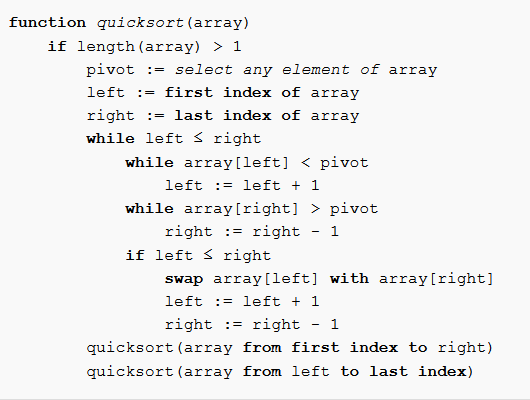
\includegraphics{quickboy} 

}

\caption{Quicksort pseudo code (Rosetta Code n.d.)}\label{fig:quickboy}
\end{figure}

An algorithm is, in essence, a sequence of computational steps that transform the input into the output; if we approach this definition in the context of software, algorithms appears to be \emph{tools for solving a well-specified problem} (Cormen \protect\hyperlink{ref-Cormen2009}{2009}, 1). In the earliest forms, there is a vast amount of sorting algorithms like the famous \emph{Quicksort} (for a detailed introduction to Quicksort from its inventor, see Hoare (\protect\hyperlink{ref-Hoare1962}{1962})). Quicksort uses an approach called \emph{divide-and-conquer} (Mackenzie \protect\hyperlink{ref-Mackenzie2006}{2006}) which enables the algorithm to divide the problem into smaller parts, find micro solutions and then combine the solutions to create the requested output. For example, if we feed Quicksort with the following array:

\[\begin{array}{ccccccc}
 2 & 5 & 7 & 4 & 3 & 1 & 6\\
.
\end{array}\]

Quicksort firstly chooses a pivot number\footnote{The method to choose a pivot decided by the coder, it can be the median of the first and last items in the array, a random item or a specific one.} (it's the number \(4\) in our example) and then it moves the pivot to the end:

\[\begin{array}{ccccccc}
 2 & 5 & 7 & 3 & 1 & 6 & \textbf{4}\\
.
\end{array}\]

Then the algorithm starts to find, firstly, starting from left finds the first number that is greater than the pivot (\(5\)) and the starting from the right the first smaller number from the pivot (\(1\)) and simply swaps those. As the process continiues recursively the steps seem like below,

\[\begin{array}{ccccccc}
 2 & 1 & 7 & 3 & 5 & 6 & \textbf{4} \\
 2 & 1 & 3 & 7 & 5 & 6 & \textbf{4} \\
.
\end{array}\]

Finally, when the greater item from the left and smaller item from the right overlap each other the pivot will be inserted in the middle:

\[\begin{array}{ccccccc}
 2 & 1 & 3 & \textbf{4} & 7 & 5 & 6 \\
.
\end{array}\]

In this final form, the items on the left are smaller and the items on the right greater than the pivot. If the same process applied recursively to both sides of the pivot individually we get the completely sorted array:

\[\begin{array}{ccccccc}
 1 &  2 & 3 & 4 & 5 & 6 & 7 \\
.\end{array}\]

Quicksort is one of the most basic examples, but it enables us to see the components of a simple algorithm. As Kowalski (\protect\hyperlink{ref-Kowalski1979}{1979}) notes algorithms consist of 2 parts, namely, \emph{Logic} and \emph{Control}. While logic component includes the knowledge to solve the problem like in the example of Quicksort what a sorted list is (i.e., A is a sorted list of B if it is a permutation of B and an arranged array at the same time)(cf. Frühwirth and Abdennadher \protect\hyperlink{ref-Fruxfchwirth2011}{2011}, 7), how do we define if one number is greater than another one or the definition of the \emph{problem} (that the array is not sorted). The second part, the control component, defines which strategy will be used to obtain the requested output(cf. Kowalski \protect\hyperlink{ref-Kowalski1979}{1979}, 425). In this sense, algorithms are deploying an agency to a certain extent on the entered data through their decision-making process based on the coded assumptions that we call logic. In the computing process, algorithm firstly arranges (or reduces) the dataset to a form that can be processed with the algorithm's logic construction and operates it with the steps of its control instructions recursively until the expected outcome is achieved.

\hypertarget{collection}{%
\section{Collection}\label{collection}}

\[ \textbf{Input/Sensor} \Rightarrow Database 1 \Rightarrow \qquad [...]\]\footnote{The notations follow the process of an algorithmic selection/recommendation as described on Figure \ref{fig:AlSel} to mention which phase of algorithmic governance that specific part of the paper is referring to.}

The digital age brought myriad ways to data collection. While nearly all public activity produces records, document archives; on an individual basis, every activity on the digital network from logging into a web service to clicking on a link leaves traces (cf. Gillespie, Boczkowski, and Foot \protect\hyperlink{ref-Gillespie2014}{2014}, 170). The first stage that makes algorithmic surveillance possible is the collection of the \emph{raw data}. The raw data was already in the interest of governments, companies, scientists for varying reasons from security to sales efficiency, to research from the very beginning of the digital age. However, the methods of data collection have been changed radically with the emergence of a more participatory internet form, namely as Tim O'Reilly(\protect\hyperlink{ref-Oreilly2009}{2009}) called it, \emph{WEB 2.0}. WEB 2.0 refers to the contemporary web structure where the users also participate as content creators through social media platforms which built upon increased personal information flows (Zimmer \protect\hyperlink{ref-Zimmer2008}{2008}, 4). Insofar, other than the automatically logged traces like logins, surf history, online purchase or sensor-based data collection like GPS logs, Radio-frequency identification (RFID) scans, fitness-tracker records, a considerable amount of data about individuals, be it social media posts or use of online communication tools, are collected from the willingly shared information. Once painfully hard work for data collection became an automatically monitored and updated process (Cheney-Lippold \protect\hyperlink{ref-Cheney2017}{2017}, 118), from which the data piles are transferred automatically into \emph{data warehouses} (cf. Rouvroy, Berns, and Libbrecht \protect\hyperlink{ref-Rouvroy2013}{2013}, 6).

\hypertarget{indexes-and-the-rule-of-data}{%
\section{Indexes and the Rule of Data}\label{indexes-and-the-rule-of-data}}

\[ Input/Sensor \Rightarrow Database 1 \Rightarrow \qquad [...]\]
\[    \qquad \qquad \qquad \qquad \qquad \qquad \qquad\qquad\qquad\qquad\qquad\qquad \qquad \Uparrow \]
\[ \qquad \qquad \qquad \qquad\qquad\qquad\qquad \qquad \qquad \qquad \qquad \qquad \qquad  \textbf{Database 3} \]

As the internet grew into a giant content reactor, the deliverance of relevant content to the users became the primary issue. This obstacle has especially hurdled search engines. The general approach of search engines to the websites is to promote the \emph{link-rich} nodes over \emph{link-poor} nodes in order to deal with the vast complexity of web links (Stalder \protect\hyperlink{ref-Stalder2009}{2010}). Google's successory PageRank's innovation that gave the algorithm the edge over the predecessors was assigning more \emph{worth} to the links from a higher ranked webpage than a link from a lower ranked webpage in the calculation of \emph{importance} (Rieder \protect\hyperlink{ref-Rieder2012}{2012}, 1); PageRank especially focuses on the worth of the incoming links to the webpage to determine its importance. The idea goes back to the origins of Eugene Garfield's Scientific Citation Index (SCI) which was simply the division of the number of citations a journal get with the number of articles they have published (Cardon \protect\hyperlink{ref-Cardon2013}{2013}, V). Soon, Pinski and Narin(\protect\hyperlink{ref-Pinski1976}{1976}) published a weighted version of the formula which also constitutes the basis of the Pagerank algorithm (see Figure \ref{fig:Narin}) that generated by the Stanford Students Sergey Brin and Larry Page. As the amount of citations delivers an approximation of the worthiness of an academic paper, the hyperlinks to a website, weighted with the linking webpage's self-worth, will be counted as a vote for the worthiness of a website (cf. Cardon \protect\hyperlink{ref-Cardon2013}{2013}, IX).

\begin{figure}

{\centering 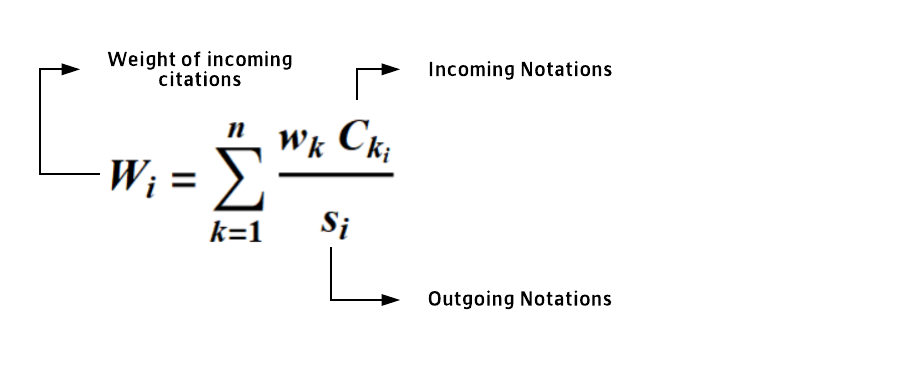
\includegraphics{Narin} 

}

\caption{Citation influence formula for scientific publications (Rieder 2012)}\label{fig:Narin}
\end{figure}

Despite its tendency to create link monopoly and creating a hyperlink market where \emph{worthy} webpages commodify their vote potentials, PageRank has indexed and weighted the whole internet for the optimization of the search results. However, solely indexing and ranking the webpages is a one-dimensional method; it creates the search results without the consideration of the individual interests. The growing information flow made the one-dimensional approach limited, as without personalization too much irrelevant information overfloods the end results. To achieve \emph{the perfect recall} (Zimmer \protect\hyperlink{ref-Zimmer2008}{2008}) on search engines, the algorithmic system needs to \emph{understand} users' intellectual wants and desires. Search engines, therefore, are also including user's digital journey as a \emph{second index} (Stalder \protect\hyperlink{ref-Stalder2009}{2010}) to personalize the search results, which eventually means monitoring and processing users' digital traces. In order to improve profiling, Google, for example, has unified the collected data from their all services, as well as different user accounts on different services to categorize the individuals on a whole different level (cf. Tsukayama \protect\hyperlink{ref-Tsukayama2012}{2012}). As the Table \ref{tab:abc} shows, today, the dominant business model of the internet giants have eventually become advertising\footnote{For a comparison, 86.78\% of Google's revenue between 2017 and 2018 was from advertising (Rosenberg \protect\hyperlink{ref-Rosenberg2018}{2018}).} and advertisers are not interested in creating better search results or a better information network on the internet but in the profiles of the users. In this sense, while search engines aim to deliver more relevant search results, \emph{to deliver relevant users to the advertisers} (Stalder \protect\hyperlink{ref-Stalder2009}{2010}) became the business model of the internet companies.

\[ Input/Sensor \Rightarrow \textbf{Database 1} \Rightarrow \qquad [...]\]

The increasing value of personal data has prepared the ground for the competition among the web corporates in the first decade of the 2000s. John Cheney-Lippold (\protect\hyperlink{ref-Cheney2017}{2017}) notes the day when Google bought the targeted-advertising corporate \emph{DoubleClick} as the beginning of the \emph{data wars}. While Google previously had only access to the users' search history and email accounts the purchase of DoubleClick enabled access to the history of the visited pages as well as the timeframe of every visit. As Google was obtaining an internet-wide surveillance power, other internet giants were trying to cope with Google's \emph{coup d'ata} (cf.~ibid. 19-20). If we take Google's data collection today as example; every click made on any of the Google's servers delivers the standard log information about the user (IP address, location, date, time, time zone, language, operating system, and browser) but Google also follows the users all around the web through the web pages which happen to have Google's DoubleClick cookies embedded, additionally Google also adds scripts and web beacons on the websites that when loaded with the webpage deliver user's information to their servers (Dover \protect\hyperlink{ref-Dover2008}{2008}). As Google's and other internet-based companies' central revenue became the advertisement, data has rapidly become the central commodity of digital capitalism, surveillance on users became the determinant factor of a successful company.

\begin{table}[t]

\caption{\label{tab:abc}Algorithmic selection in top 10 websites (cf. Just and Latzer 2017, 250)}
\centering
\begin{tabular}{lll}
\toprule
Ranking & Website & Primary use of algorithmic selection\\
\midrule
1 & google.com & General search engine, Computational advertising\\
2 & facebook.com & Computational advertising\\
3 & youtube.com & Computational advertising\\
4 & baidu.com & General search engine, Computational advertising\\
5 & yahoo.com & General search engine, Computational advertising\\
\addlinespace
6 & amazon.com & Special search, Recommendations, Reputation (sellers)\\
7 & wikipedia.org & Special search engine\\
8 & qq.com & General search engine, Computational advertising\\
9 & taobao.com & Special search, Recommendations, Reputation (sellers)\\
10 & twitter.com & Computational advertising\\
\bottomrule
\end{tabular}
\end{table}

\begin{figure}

{\centering 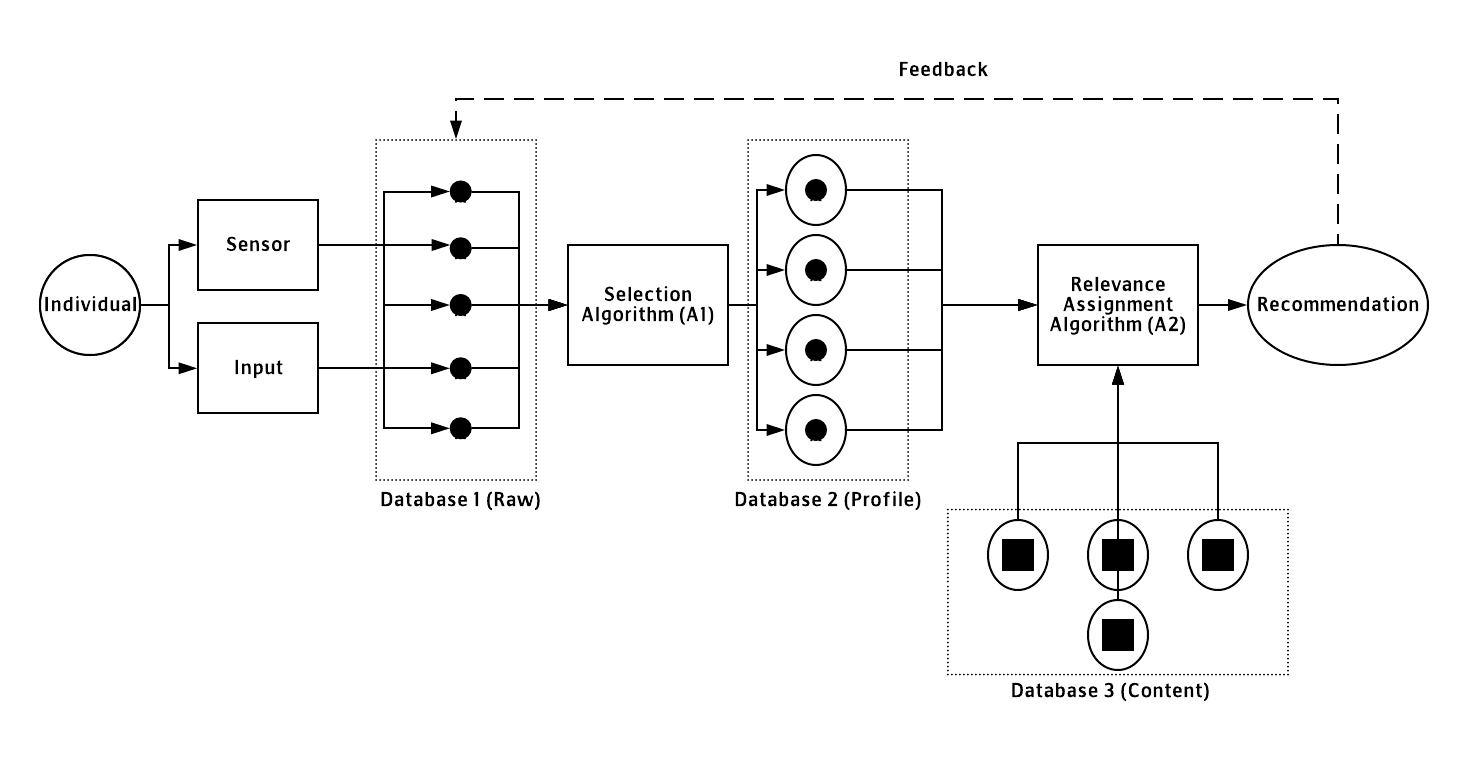
\includegraphics{AlSel} 

}

\caption{Algorithmic Selection Process (cf. Just and Latzer 2017, 241)}\label{fig:AlSel}
\end{figure}

\hypertarget{categorization}{%
\section{Categorization}\label{categorization}}

\[Input/Sensor \Rightarrow Database 1 \Rightarrow \textbf{Sel. Algorithm (A1)}  \Rightarrow  Database2 \Rightarrow \qquad [...]\]

The collected data is unsorted and heterogeneous in its first stage, lacks any subjectivity. To obtain knowledge from the databases, the data needs to be processed through certain steps of statistical analysis. \emph{Data mining} process, therefore, is a pursuit of knowledge production by finding patterns and subtle correlations in the data (Rouvroy, Berns, and Libbrecht \protect\hyperlink{ref-Rouvroy2013}{2013}, 176). The vast data piles, today's colossal input flow creates, are mostly unintelligible to the traditional data processing software. In order to create knowledge, the process needs to be automated through algorithmic processes. The notion of \emph{big data}, therefore, does not tell much by itself; it is the reciprocal relation with algorithms that gives huge data piles \emph{purpose and direction} (Beer \protect\hyperlink{ref-Beer2017}{2017}, 3).

Algorithmic processes that web analytics, online store, social media, and search engine firms use, are processing the user's online history and other tracked data to create a profile. These profiles, algorithmically created identities constitute the basis for the next steps of the process like what kind of recommendations, advertisements the user will get or what kind of information will be filtered from her (see Figure \ref{fig:AlSel} for an illustration of the process). Data, therefore, first needs to be interpreted through an algorithmic system for categorization in order to model a profile for the individual. In this process, first, the collected data about the individual will be reduced to an intelligible form by the software, data particles of the individual will be \emph{vectorized}; and second, these vectorized particles will be brought together to form a processable profile of the individual which can be associated with specific content to create a personalized end result. In the earlier database formations, the categorization was a strict process; data were categorized in an inflexible and hierarchical way (Gillespie, Boczkowski, and Foot \protect\hyperlink{ref-Gillespie2014}{2014}, 171). However, algorithmic systems today, that handle the selection, do not have necessarily static categories in which they simply insert users' data; in contrary, the code is in a dynamic relationship with the reality and the determination of the categories bound to the underlying logic of the algorithms. John Cheney-Lippold ((\protect\hyperlink{ref-Cheney2017}{2017}) \& (\protect\hyperlink{ref-Cheney2011}{2011})) aims explicitly for the question, what a \emph{norm} means for an algorithmic system with the example of gender as a category;

\begin{quote}
{[}\ldots{}{]} algorithms allow a shift to a more flexible and functional definition of the category, one that de-essentializes gender from its corporeal and societal forms and determinations while it also re-essentializes gender as a statistically-related, largely market research-driven category. Gender becomes a vector, a completely digital and math-based association that defines the meaning of maleness, femaleness, or whatever other gender (or category) a marketer requires.

--- (Cheney-Lippold \protect\hyperlink{ref-Cheney2011}{2011}, 170)
\end{quote}

\[ [...] \Rightarrow Sel. Algorithm (A1) \Rightarrow  \textbf{Database 2} \Rightarrow Rel. Ass. Algorithm (A2) \Rightarrow Recommendation\]
\[   \qquad \qquad \qquad \qquad \qquad \qquad \qquad \qquad \qquad \Uparrow \]
\[ \qquad \qquad \qquad \qquad \qquad \qquad \qquad \qquad \qquad Database 3 \]

The categories of the profile, where the collected data particles of user stored, will be continuously updated and rearranged as the new data about her behavior is received, e.g., a \emph{person X} who has been identified as \emph{female} can be redefined as a \emph{male} if her online habits appear to be more \emph{male-like} in the latest feedback. In this loop, as the more data arrives in the system, the more precise the categorization will be (cf. Cheney-Lippold \protect\hyperlink{ref-Cheney2011}{2011}, 168--70). However, precision does not mean necessarily that the digital gender of the individual will be aligned to her real-life gender with more data. Maleness is not a fixed category that is defined through specific qualities from the real world, rather than, maleness is an average that the algorithmic process extracts from the activity habits of a specific population. For example, if Google's category \emph{male} defined as someone who gets his news from the websites A, B and shops on the website C while enjoys the music of the Band D, the individual whose habits fits into this criteria will be defined as male; if the habits of the individual overlaps into the category of \emph{female} than the identity can also be defined, for example, as 80\% male/ 20\% female (cf. Cheney-Lippold \protect\hyperlink{ref-Cheney2011}{2011}, 180). As the user's digital identity gets realigned with the new data, the category itself also will be redefined through the demographic changes in the behavior of its population (cf. Cheney-Lippold \protect\hyperlink{ref-Cheney2017}{2017}, 59--61). If the greater part of the individuals who have been defined as male show different habits than the algorithmic expectation (e.g., visiting the website E as the news resource instead of B), the category \emph{male} will be altered in the process. The flexible categories of \emph{gender}; therefore, do not specifically have pre-assumptions about the nature of maleness, it does not lock the user's digital experience into a pre-determined process. The categories are not carrying the purpose of mapping reality but to create the most effective and functional way to model human behavior (cf.~ibid., 137-141). This flexibility in the code, however, is hard to achieve for the traditional step by step method of programming algorithms as the complexity of the data rises; therefore, new selection structures especially built and enhanced on semi- or unsupervised \emph{learning} algorithmic systems that brings automation on a different level.

\hypertarget{learning-machine-and-the-invisible-gambit}{%
\section{Learning Machine and the Invisible Gambit}\label{learning-machine-and-the-invisible-gambit}}

Van Otterlo defines machine learning(ML) as \emph{a branch of AI that seeks to develop computer systems that improve their performance automatically with experience} (Van Otterlo \protect\hyperlink{ref-Otterlo2013}{2013}, 46). The ML approach has become the technical basis of the data mining process (Witten et al. \protect\hyperlink{ref-Witten2016}{2016}, XIII). The logic behind ML aims to solve the problems for the situations where we do not have a simple algorithmic solution. Ethem Alpaydın (\protect\hyperlink{ref-Alpaydin2004}{2004}) gives the example of spam mails; we cannot specifically define what a spam mail is and/or code it for an algorithmic process to recognize considering that the definition of the spam mail changes from time to time or individual to individual. However, we can show an enormous amount of different spam mails if we somehow get the algorithmic system to conceptualize an image of a spam mail with the training by given examples. Therefore, the ML is a clever way to compensate \emph{what we lack in (computing) knowledge with the data} (ibid. 1). If we turn back to the simple example of the Quicksort, ML approach would exclude the logical base that constitutes Quicksort's understanding of what a sorted array is, instead, it would get the algorithm to figure out the nature of a sorted array by showing countless different examples of sorted arrays and let algorithm to build its own control scheme (instead of the step by step code example on the Figure \ref{fig:quickboy}) to turn an unsorted array to a sorted one, thus, what kind of reasoning algorithm builds to define a sorted array stays a mystery.

ML algorithms constitute an effective basis for the search engine and social media companies that have an enormous amount of data about individuals and are struggling to continually develop algorithms that can govern the data. In this direction, Google is already replacing the PageRank algorithm with the ML algorithm BrainRank (Schachinger \protect\hyperlink{ref-Schachinger2017}{2017}) while Facebook is vehemently replacing all of its algorithmic background with unnamed ML algorithms since a while (McGee \protect\hyperlink{ref-McGee2013}{2013}). However, ML algorithms are extending the opacity of the decision-making process even further. The black box structure of the algorithms can be addressed with a few different layers of struggle. The first layer of the opacity is caused by technological illiteracy, most of the users are not aware of the algorithmic decisions on the background, nor they can analyze the code; the second layer is the unwillingness of the companies to share the details about their algorithmic processes (Stalder \protect\hyperlink{ref-Stalder2009}{2010}), most of the information about algorithmic systems of the internet service companies are figured out through the analysis of inputs and outputs or by observing other similar examples; the third layer is the complexity of algorithmic systems, after the collective work of large quantity of the programmers the algorithmic system might become unintelligible even for the individual programmers who work in the coding process (cf. Pasquale \protect\hyperlink{ref-Pasquale2015}{2015}, 6); and finally the algorithmic structure, ML approach produces, completely blurs the functioning body of the software, since the ML algorithm creates its own control process, even its designers are only able to observe the input and output, therefore, it is entirely invisible to the individuals how the ML process produces knowledge (Rouvroy, Berns, and Libbrecht \protect\hyperlink{ref-Rouvroy2013}{2013}, VII). A great example of the self-learning opacity is Google's latest ML Chess Algorithm \emph{AlphaZero}. AlphaZero learned to play chess by training on a vast database of previously played chess games and it took AlphaZero 4 hours of training to beat the previously unbeaten chess algorithm \emph{Stockfish 8} in a 100 game tournament by 28 wins, 0 losses, and 72 draws (Silver et al. \protect\hyperlink{ref-Silver2018}{2018}, 4--5). The strange thing in the process was that AlphaZero preferred a specific chess opening, namely, the \emph{Queen's Gambit} (QG) pretty highly in its training and gained more success with it than any other opening style (ibid., 3). Considering the professional chess plays between humans since 1950 QG opening is fourth popular opening style (Olson \protect\hyperlink{ref-Olson2014}{2014}) and as we get to the tournament games between grandmasters it is an even rarer sight to see this particular opening. AlphaZero, now the world's best chess player, saw a probabilistic advantage in the QG game that chess grandmasters did not see since the beginning of the history of chess. If it is because a safer way to play or delivers a particular advantage for the end game cannot be discovered by the programmers of AlphaZero or any other person by looking at the code of the algorithm.

\begin{figure}

{\centering 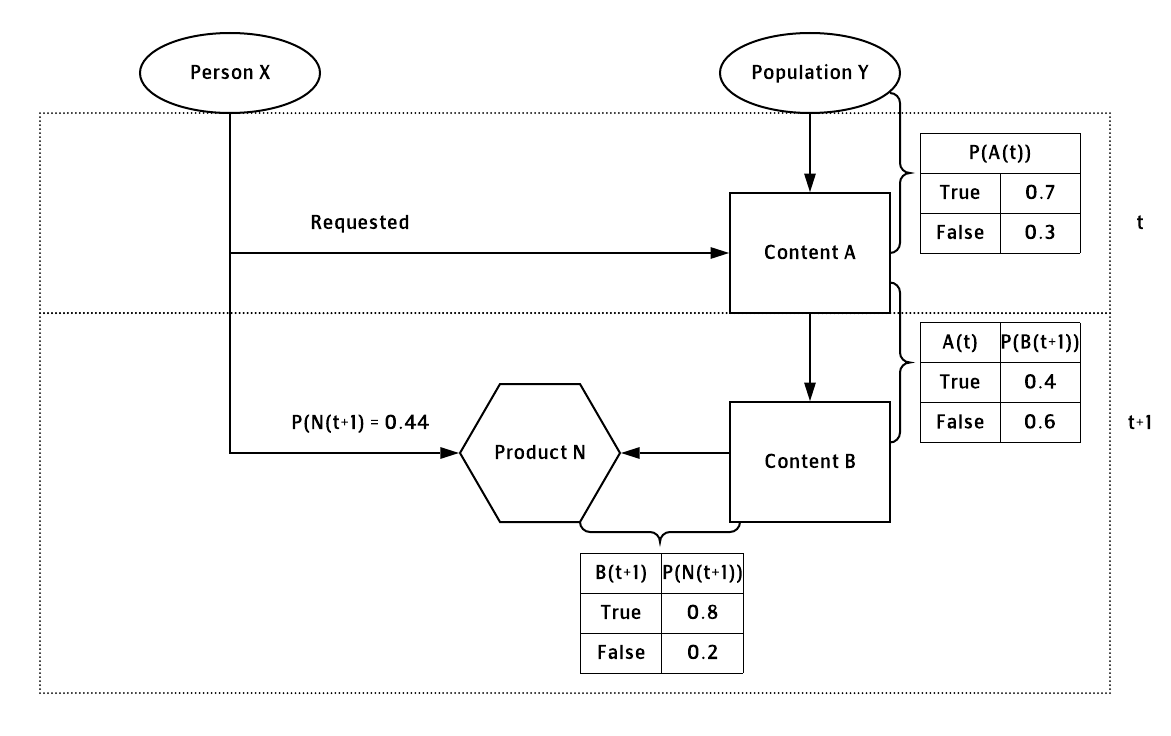
\includegraphics{Bay} 

}

\caption{A simplified example of a dynamic Bayesian network (cf. Van Otterlo 2013, 50)}\label{fig:Bay}
\end{figure}

\newpage

\[ [...] \Rightarrow Sel. Algorithm (A1) \Rightarrow \ Database 2 \Rightarrow \textbf{Rel. Ass. Algorithm (A2)} \Rightarrow Recommendation\]
\[   \qquad \qquad \qquad \qquad \qquad  \qquad \qquad \qquad \Uparrow \]
\[ \qquad \qquad \qquad \qquad  \qquad \qquad \qquad \qquad Database 3 \]

As mentioned above in the example of AlphaZero, ML algorithms are \emph{learning} through creating probabilistic network structures on the dataset. Therefore, the algorithmic selection process associates the profiles of the individuals with the content that will be fed into the individualized search results, marketing ads, social media posts in the same manner. Profiles will get fit into joint models such as Martjin Van Otterlo (\protect\hyperlink{ref-Otterlo2013}{2013})'s example of \emph{Bayesian networks}. Bayesian network is one of the modeling techniques ML algorithms use to assign relevance through a probabilistic connection network between different indexes, profiles (cf. Van Otterlo \protect\hyperlink{ref-Otterlo2013}{2013}, 49); as the simplified example of connection on Figure \ref{fig:Bay} shows the network consists of nodes which through arrows indicate probabilistic connections among them which enables the calculation of the \emph{joint probabilities} (cf.~ibid.). As shown on the Figure \ref{fig:Bay}; if we follow a targeted product advertisement an online shopping webpage like \emph{Amazon} would contain, when the \emph{Person X} requests a search result, social media post or a news article of \emph{Content A} her profile will be probabilistically associated to the prolific populations that also made the same request (on the simplified example \emph{Population Y} associated to \emph{Person X} because of the high probability of the same choice among the \emph{Population Y} but on a complex model association would be made through the correlations of varying parameters). After that, the \emph{Population Y}'s following requests after the request of \emph{Content A} will directly determine the probability of the recommendations \emph{Person X} will get. As the given example on the figure the individuals on the \emph{Population Y} that requested \emph{Content A} will request \emph{Content B} with a probability of \(0.4\) based on the further informations population's probability of buying the \emph{Product N} (which is in an association with the \emph{Content B}) can be calculated as \(0.44\)\footnote{Given that we are calculating the part of the \emph{Population Y} that visited \emph{Content A} at the time \emph{t}, the summation of the probabilities of the purchase of \emph{Product N} with the request of \emph{Content B} at \emph{t+1} (\(0.4*0.8\)) and the purchase of \emph{Product N} with the request of \emph{Content B} at \emph{t+1} (\(0.6*0.2\)) shows the probability of the purchase of \emph{Product N} in the part of the population that requested the \emph{Content A} at \emph{t}.} which will shape the probabilistic assumption of the \emph{Person X} buying \emph{Product N} without having any personal connection to \emph{Content B}. The personalized results and recommendations \emph{Person X} will receive are, therefore, directly connected with the population(s) she has been associated with. The Bayesian network is only one of the approaches to build such connections, there are different examples of similar probabilistic network schemes as well as alternatives to the deductive reasoning, however, the general logic of a ML environment stays the same as the connection between the entities on the representation will be solely connected to their probabilistic alignments.

Algorithmic modeling, in this sense, does not work to map the reality (Vieth and Wagner \protect\hyperlink{ref-Vieth2017}{2017}, 11), the data mining process is not about finding the underlying causations of the human behaviour as the classical statistical analysis was aiming to do through modeling the real world data and creating hypotheses to test with it (Rouvroy, Berns, and Libbrecht \protect\hyperlink{ref-Rouvroy2013}{2013}, VIII-IX). ML algorithms are not specifically testing a hypothesis through the data; on the contrary, they are creating their own hypotheses in the process of analysis. The knowledge production relies solely on correlations (ibid.), sterile from the discussion about causation. As Georg E.P. Box(\protect\hyperlink{ref-Box1987}{1987}, 424) once famously stated \emph{all models are wrong but some are useful}, modeling has been the central methodology for creating knowledge about human behavior and the external world. The \emph{datalogical turn} (Clough and Gregory \protect\hyperlink{ref-Clough2015}{2015}) with the emergence of the internet and the algorithmic power made it possible to work without models. Anderson (\protect\hyperlink{ref-Anderson2008}{2008}) mentions the example of Google's takeover of the advertisement sector. When Google decided to enter the advertisement sector Google's counterparts were still using behavioral, cultural models and sticking to the conventional advertising tools. Google relied solely on extensive data and better analytical tools. In the end, finding correlations in the vast data files through statistical algorithms bested Google's counterparts and their modeling techniques. Turns out, tracking and measuring enough amount of data works better to predict human behavior than to searching for causality and modeling to answer the question why people do what they do (cf.~ibid.).

\newpage

\hypertarget{anchors-and-endless-while-loops}{%
\section{Anchors and Endless While Loops}\label{anchors-and-endless-while-loops}}

\[ [...]\Rightarrow \ Database 2 \Rightarrow Rel. Ass. Algorithm (A2) \Rightarrow \textbf{Recommendation}\]
\[    \Uparrow \]
\[  Database 3 \]

\begin{quote}
{[}\ldots{}{]} personalization filters serve up a kind of invisible autopropaganda, indoctrinating us with our own ideas, amplifying our desire for things that are familiar and leaving us oblivious to the dangers lurking in the dark territory of the unknown.

--- (Pariser \protect\hyperlink{ref-Pariser2011}{2011}, 13)
\end{quote}

The automated process makes the decision which variables, observations are more likely to be seen in the future or which variables are more likely to have a relation (Cf. Vieth and Wagner \protect\hyperlink{ref-Vieth2017}{2017}, 20). The probabilistic network built upon the users' profile creates a digital reality through the suggestion algorithm refers through its means of inference. Following Eli Pariser's quote; algorithmic processes are seemingly taking user's previous habits as the basis of their decision-making process. However, is the digital reality created at the end is not just the \emph{amplification} of personal features? To answer this question, one needs to analyze which factors are skewing the end results algorithmic processes seemingly offer.

John Cheney-Lippold (\protect\hyperlink{ref-Cheney2011}{2011}) uses the term \emph{cybernetic categorization} to define the flexible categories managed by ML algorithms to constantly (re)define user profiles (ibid. 171). \emph{Cybernetics}, the term that first coined by the mathematician and philosopher Norbert Wiener (\protect\hyperlink{ref-Wiener1948}{1948}), is a transdisciplinary approach to study the operation and learning patterns in the human and animal brains in order to mimic the same reasoning in the operation of the machines. The word \emph{kybernetes} means steersman and its Latinization \emph{gubernator} is the root of the term \emph{government} (cf.~ibid. 14-15). As the name indicates, the cybernetical logic follows the art of steering and the act of steering is achieved through feedback loops between the environment and the \emph{subject}. For example, a rat that seeks the cheese in a maze will receive feedback from its environment whenever it gets stuck in a dead end, thus, next time the rat will steer its direction closer to the way to the cheese and as the number of trials advance it will alter its behavior in a way that will successfully lead to the cheese (cf. Corning \protect\hyperlink{ref-Corning1996}{1996}, 105). Modern robotics conceptualized this approach as the sense-think-act loop where a simple robot will \emph{sense} its environment through its sensors, \emph{think}/ analyze the feedback and steer the behavior through statistical inference, and \emph{act} in the newly calculated way until the new feedback arrives (cf. Siegel \protect\hyperlink{ref-Siegel2003}{2003}).

\[[...] \qquad \qquad \qquad \Leftarrow   \qquad \qquad   \textbf{Feedback} \]
\[    \qquad  \qquad \qquad \qquad \qquad \qquad \qquad \Uparrow \]
\[ [...]\Rightarrow Rel. Ass. Algorithm (A2) \Rightarrow Recommendation\]

Cybernetic categorization, therefore, an anchoring system of the categories to the constant data flow that extracted from the subject, the reciprocal feedback loops in this process steer the profile in more \emph{effective} forms of profiling that will enable to map the individual's interests, desires in a to predict future behavior in the algorithmic selection process, which this section specifically aimed to explain. However, if we look at the process of algorithmic governance as a process of creating a personalized digital reality as Just and Latzer (\protect\hyperlink{ref-Just2017}{2017}) mention, there are more than one feedback loop that fuels the machinery. First as have been mentioned, on the category level, the categories will be updated as the new data arrives; however, the feedback loop on the level of categories is only one side of the anchoring process, namely, the anchoring of the algorithmically produced results to the user's previous behavior. Second anchoring is between the subject's profile and the population her profile is categorically identified with; the subject's algorithmically created digital reality will be continuously steered to the direction of the specific populations. With other words, the content our subject gets will be filtered to fit into the behavior of specific \emph{alignments}, where the content will be shaped firstly according to the previous behavior and secondly with the habits of the categorically associated populations. Following the same direction, the third feedback loop stands between the subject and the digital reality. As the information the subject gets filtered, personalized by the two anchoring systems in the machinery subject's behaviour and thinking will also steered in alignment with the entities her digital identity associated with and the steered behaviour, as in the example of the robotics, will be shaped through the experience and feed the process with the new, relatively \emph{normalized} behaviour, creating the third feedback loop.

\hypertarget{hob}{%
\chapter{Hobbit and the coils of the serpent}\label{hob}}

\begin{center}\rule{0.5\linewidth}{\linethickness}\end{center}

In the J.R.R. Tolkien (\protect\hyperlink{ref-Tolkien2009}{2009})'s \emph{The Lord of the Rings} the main antagonist Sauron exists only in the form of a panoptic gaze. His manifestation on the \emph{Middle Earth} is a lidless eye that gazes from the top of \emph{Barad-dûr}, the dark tower (ibid. 942). Sauron's actual power seems to be reserved in the \emph{One Ring} but Tolkien specifically do not describe exactly what powers Sauron's eye or the \emph{One Ring} have. The Eye stays as an obscured gaze, as a limitless surveillance source over the Middle Earth. However, there is another artifact in which Sauron's will appears to be expressed, the \emph{Palantír} (ibid. 597). The \emph{Palantírí} are black stone spheres, namely the far-seeing stones, which built for communication from great distances by the ancient elves and scattered around the Middle Earth to create an instantaneous communication network between distant realms. One of them, namely \emph{Ithil-stone} (ibid., 598) appears to be seized by the Sauron's will, and therefore whenever someone uses another one of the stones, it will be a trial against Sauron's corrupting will where the defeat means a complete subjection to Sauron's bidding. We encounter two important characters along the story who have fallen into the Palantír's influence; namely, \emph{Saruman}, the greatest mage on the Middle Earth and \emph{Denethor}, the ruling steward of \emph{Gondor}. Denethor, without knowing that he was communicating with Sauron, and Saruman, thinking he could overcome the will of Sauron, interacted with the stones, allowing Sauron to extract information through their communication and use it to influence them. Note that even Sauron is not able to lie through Palantír, but he can tell specifically selected truths to create a personalized reality to influence the subject on the other end of the communication line. Sauron's limitless surveillance power along with his ability to gain information about the individuals through the communication on Palantír eventually lures Denethor into being a fearful and broken man and Saruman into being a loyal servant by making them believe that there is no hope against the inevitable victory of Sauron's forces.

Sauron's reality construction works with the information about subjects he collects through the Palantír and the information about the Middle Earth he gains through his limitless surveillance ability. Palantír is, in this regard, a medium that brings Sauron's power beyond surveillance, turning his ubiquitous surveillance into the governance of subjects. Dataveillance combined with the algorithmic decision-making processes gains the ability to form the digital reality of the subjects in a similar manner; the whole process operates through an incomprehensible amount of data about the individual and the world that surrounds her. It is, however; as the example of Palantír indicates, not a supervisory surveillance art like in panopticism where the observer only engages if the subject does not fulfill a specific behavior pattern. The collection of the data is done automatically, and in a ubiquitous manner, the observer (or the source of observation) is obscured, the watchtower of the panoptic structure has vanished. This invisibility is not to be mistaken with the anonymity of the observer in the panoptic surveillance, even if the inmates can't observe the watchers, the expectations from the inmates are clear in the panopticon; in the digital reality, on the other hand, most of the individuals aren't even aware of the fact that surveillance is indeed happening; and even for the ones who are aware of the process, it remains as a black box on different levels of opacity as mentioned in Chapter \ref{alg}; the source of surveillance is not concealed, it is invisible. Following Antoinette Rouvroy ((\protect\hyperlink{ref-Rouvroy2013}{2013}) \& (\protect\hyperlink{ref-Rouvroy2016}{2016})), Susanne Krasmann (\protect\hyperlink{ref-Krasmann2017}{2017}) and John Cheney-Lippold ((\protect\hyperlink{ref-Cheney2011}{2011}) \& (\protect\hyperlink{ref-Cheney2017}{2017})), I find the contribution of Gilles Deleuze especially with his short essay \emph{Postscript on the Societies of Control} (\protect\hyperlink{ref-Deleuze1992}{1992}) influential to analyze the contemporary changes in the operation of power; Deleuze names the behavior patterns, disciplinary power tends to form subjectivities into, as \emph{molds} and the modern form of control on subjectivity as \emph{modulation} (ibid, 4). While the molds of the disciplinary society \emph{correct} the individuals in specific ways, today's digital process which through the algorithmic decision-making processes go beyond the surveillance by continuously modulating the \emph{reality} of the digital subject (Krasmann \protect\hyperlink{ref-Krasmann2017}{2017}) of our era. Algorithmic governance, however, does not have a specific intention behind the curtains like the disciplinary power or the Sauron's will in the Palantír's communication network, it is more interested in making the subjects \emph{knowable} (ibid. 11).

\begin{quote}
\emph{H: Algorithmic governance of the information on the web transforms surveillance into a non-disciplinary normalization exercise in alignment with Michel Foucault's definition of the characteristics of neo-liberal governmentality.}
\end{quote}

After arguing that algorithmic governance does not contain a direct disciplinary intention; following the direction of the hypothesis Foucault's notes about the transition from liberal to neo-liberal art of governance offers a further discussion about the machinery of the algorithmically governed digital network. As the digital surveillance becomes an art of governance through algorithmic selection and \emph{reality construction} (Just and Latzer \protect\hyperlink{ref-Just2017}{2017}) process through the big data as described on the Figure \ref{fig:AlSel}, it shows specific similarities to Foucault's definition of the neo-liberal governmentality. Following Foucault's argumentation; in contrast to the liberal art of governance, neo-liberal governmentality interested more in the environment of the subjects and defining it with market norms than to a direct focus on their subjectivities. Contemporary algorithmic governance operates the same mentality in its focus on forming a digital reality. The modeling of the digital environment starts with the indexing of the digital content. As the example of the PageRank shows, the content of the internet will be firstly indexed in a way that creates a link market where the \emph{worth} of the webpages becomes the object of a massive trade network and secondly the authorities that run the indexing process are the greatest advertisement companies which get most of their revenue through their advertisement services. The process follows with the indexing of the individuals to personalize the service of the digital content, in this process the individual first needs to be reduced into data bits which Deleuze calls as \emph{dividuals} (Deleuze \protect\hyperlink{ref-Deleuze1992}{1992}, 5), what makes an individual indivisible will be atomized in the process; thereafter, the data particles will be brought together to form a data double of the subject. However, in the construction of the profile in the algorithmic process, the representation of the individual is not the goal anymore, the data particles will be categorized solely to map consumer behavior without the consideration of the meaning of the features in the real world. As Felix Stalder (\protect\hyperlink{ref-Stalder2009}{2010}) argues both the content and subject itself will be categorized in a market environment because as much as the content will be delivered to the individuals, the individuals will be delivered to the advertisers. The personalization of the information that should reinforce the subject's experience becomes the commodification of the subject's data and the algorithmically created knowledge through it. In this regard, algorithmic governance shows similarity with neo-liberal governmentality in the construction of the (social - digital) environment with market norms.

Following Deleuze's concept of \emph{control}, Cheney-Lippold defines the normalization of the subject in the perpetual feedback loop between the algorithmically assigned categories and the subject as an intentional training of the body (cf. Cheney-Lippold \protect\hyperlink{ref-Cheney2011}{2011}, 168--78). However; although the connections this paper draws generally align with Cheney-Lippold's work, following Thomas Lemke's contribution to Foucault's definition of the neo-liberal governmentality by arguing that neo-liberal governmentality is not interested in normalizing the society (Lemke \protect\hyperlink{ref-Lemke2001}{2001}, 200), I argue that the normalization or solely concentrating on the cybernetic categorization do not tell the whole story about the algorithmic governance. Considering the insight Van Otterlo (\protect\hyperlink{ref-Otterlo2013}{2013}) delivers on the structure of machine learning algorithms, it appears to be that the algorithmic selection machinery anchors the user's digital experience to previous behavior and the categorical populations the individual has been continuously (re)identified with; the subject's normalization occurs through the perpetual feedback loop between her and the machinery. In those anchoring processes; however, instead of an intentional training of the body, the normalization process occurs from an assumption about the human behavior in similarity with Foucault's definition of the neo-liberal perspective on the rational subject, homo œconomicus. Neo-liberal approach to the subject assumes that the rational subject will react to the environment in a non-random way because the subject is eventually defined as a collection of interests. As the non-randomness dictates, it is only natural for the subject to be in alignment with her previous consumer behavior in the future decisions and since the subject is defined as a collection of interests, it is natural for the subject to converge into groups that align with specific interests rational subject's code indicates. Therefore, instead of training of the subject, there is an environment built upon specific assumptions about the being of homo œconomicus. Antoinette Rouvroy's notes on the predictability elaborate the situation precisely as:

\begin{quote}
In their seemingly non-selective way of relating to the world, data mining and algorithmic profiling appear to take into consideration the entirety of each reality, right down to its most trivial and insignificant aspects, putting the whole world on par -- the businessman and the charwoman, the Sikh and the Icelandic. The aim is no longer to exclude anything that does not fit the average but to avoid the unpredictable, to make sure that everyone is truly themselves.

--- (Rouvroy, Berns, and Libbrecht \protect\hyperlink{ref-Rouvroy2013}{2013}, IX)
\end{quote}

Rouvroy's argumentation can also be understood as the amplification of the specific features about the subject that have been extracted from the data as Eli Pariser (\protect\hyperlink{ref-Pariser2011}{2011}) argues, not in order to make subjects intentionally \emph{themselves} but assuming they are always already themselves because of the non-random, predictable reasoning of economic rationality of homo œconomicus that is built on an array of interests. I find Foucault's definition of the neo-liberal governmentality as defining environment and subject's relationship with the environment through a set of assumptions without specifically aiming for the training of the individual more in alignment with the structure of algorithmic governance in comparison to an intentional \emph{control} exercise on the subjectivity.

The increasing levels of opacity in the algorithmic governance process that have been mentioned in Chapter \ref{alg} are also worth mentioning in comparison with the neo-liberal governmentality. As the black box structure of the algorithms increases, the process seems more natural to the users, \emph{modulated} digital reality stays in the level of \emph{technological unconscious} (Thrift \protect\hyperlink{ref-Thrift2004}{2004}). The tendency of the neo-liberal governmentality to alter the reality of its subjects also aligns with the natural (and therefore objective) appearance of the algorithmic selection processes. In Gary Becker's definition homo œconomicus mentioned in Chapter \ref{theory} is someone who accepts the reality and reacts to it with her economic rationality, however, the reality the subject excepts is an object of the surrounding governance structure, especially in neo-liberal governmentality there is a direct intention to form the rules of that reality. In this sense, the natural appearance of the changes in the homo œconomicus' environment is a reinforcing feature in the neo-liberal art of governance. Although this paper does not seek methods to change the contemporary operation structure of the algorithmic governance, critical approaches against algorithmic governance are turning from methods to enhance data privacy to technologies to enhance transparency (Van Otterlo \protect\hyperlink{ref-Otterlo2013}{2013}, 57) of the algorithms.

Finally, on an additional point, as neo-liberal governmentality tries to reduce societal relations to a specific simplicity in order to represent them in economic analysis as mentioned through Lemke's notes in Chapter \ref{theory}, the relations between subjects and populations will be represented as probabilistic connections in the algorithmic governance as explained with ML algorithmic structures in Chapter \ref{alg} with the example of the Bayesian networks. The tendency in algorithmic governance is to bloat the volume of data to increase accuracy as much as possible. While it has been proven to be an effective way to build a predictive advertisement environment, it completely denies creating knowledge about the causality of human behavior and social relations. Defining individuals solely through their specific discrete interests of their consumer behavior carries a risk. Turning back to the example of Palantír, after Sauron realizes that the ring bearer is a hobbit that travels with a peculiar party, Sauron actively seeks him. After our party encounters one of the Palantírí; Sauron, realizing there is a hobbit in the near of the stone, quickly sends his tempting call through the Palantír. However, the hobbit that falls into the temptation of the stone is not the ring bearer but another one of the four hobbits in the party, namely, Pippin (Tolkien \protect\hyperlink{ref-Tolkien2009}{2009}, 591). After Sauron extracts as much information as he can from Pippin, being sure he found the ring bearer, Sauron turns his gaze to Pippin's party. Therefore, after the real ring bearer Frodo and his companion Samwell split up from the party, they remain undetected until it is already too late for Sauron. Despite his ability to limitless surveillance Sauron was only interested in specific features of the ring bearer, he was not interested in the meaningless characteristics of Frodo. His calculation of likelihood through the categories about the ringbearer like that he is a hobbit and travels with the mage, elf, and dwarf indicated a high probability about Pippin being the one he was looking for. This false positive eventually caused Sauron's doom. While humans are generally not good at understanding the long term probabilistic connection like our inability to completely comprehend the what advantage AlphaZero finds in its favorite playing styles there is also an inaccuracy to represent the information about human behavior solely on a network of probabilistic connections.

\hypertarget{conclusion}{%
\chapter{Conclusion}\label{conclusion}}

\begin{center}\rule{0.5\linewidth}{\linethickness}\end{center}

This paper started with questioning the biopolitical meaning of contemporary algorithmic governance structure on the internet. After mentioning Michel Foucault's thoughts on the surveillance in the disciplinary societies with his concept of Panopticism, the Chapter \ref{theory} mainly dealt with the difference between the liberal and neo-liberal art of government mentioned in Foucault's later works which deliver a comprehensive discussion about the modern transitions in the exercise of power. Foucault's notes on the differences the neo-liberal governmentality brought over its liberal counterpart like the focus on shaping environment instead of individuals, definition of the social life through the economic principles, tendency to reduce the rationality and human behaviour to an intelligible simplicity enabled me to form a theoretical basis for the further discussion about algorithmic governance.

After attempting to define algorithms and discussing the short history of the digital surveillance Chapter \ref{alg} continued with the definition of the algorithmic selection process that defines the nature of the information flow the subjects of our digital era get. Analysis of the categorization, profiling, relevance and suggestion processes of the algorithmic surveillance enabled me to argue that firstly the digital reality created by the algorithmic processes anchors the perpetual information flow between the subject and the algorithmic medium firstly to the data about subject's previous behavior and secondly to the population subject's digital profile continuously (re)identified with which canalizes subject's behaviour into specific alignments as the feedback loop between the subject and algorithmic system continue.

After additionally mentioning the specific characteristics of the algorithmic governance like the opacity in the algorithmic machinery as well as the new advancements like machine learning approach in the Chapter \ref{alg}, following Chapter \ref{hob} aimed to constitute a comprehensive interpretation of the mentioned features of the algorithmic governance with the theoretical basis constructed on the Chapter \ref{theory}. The main interpretation line in Chapter \ref{hob} discusses algorithmic governance with Foucault's theory on a few points. Firstly; contrary to the operation of the disciplinary power, algorithmic governance does not seem to be interested in specific training on the subjectivity; it also does not show the characteristics of the panoptic structure as the observation itself becomes entirely opaque without making pressure on the subjects through omnipresent visibility, secondly; the formation of the information flow on the internet under the algorithmic governance that exists mainly as an advertising-oriented environment shows tendencies to the neo-liberal govermentality's pursuit to define social sphere through market norms, thirdly; although not disciplinary algorithmic governance still deploys a normalization effect on the subjects by anchoring their digital experience firstly to their previous behavior and secondly to the categorical populations they have been continiously (re)identified with, this alignment process seems to be based on the same assumptions on the human behaviour in neo-liberal governmentality by defining the rational subject \emph{homo œconomicus} as a non-random reactioning subjectivity which is only defined through a collection of interests, thus, assuming that the behavior of the subject should naturally align with the previous decisions as well as with the population that shows a similar interest as the subject.

\hypertarget{references}{%
\chapter*{References}\label{references}}
\addcontentsline{toc}{chapter}{References}

\begin{center}\rule{0.5\linewidth}{\linethickness}\end{center}

\hypertarget{refs}{}
\leavevmode\hypertarget{ref-Alpaydin2004}{}%
Alpaydın, Ethem. 2004. ``Machine Learning.'' \emph{Massachusetts Institute of Technology, USA}.

\leavevmode\hypertarget{ref-Anderson2008}{}%
Anderson, Chris. 2008. ``The End of Theory: The Data Deluge Makes the Scientific Method Obsolete.'' \emph{Wired}. \url{https://www.wired.com/2008/06/pb-theory/} (January 29, 2019).

\leavevmode\hypertarget{ref-Beer2017}{}%
Beer, David. 2017. ``The Social Power of Algorithms.'' \emph{Information, Communication \& Society} 20(1): 1--13. \url{https://doi.org/10.1080/1369118X.2016.1216147}.

\leavevmode\hypertarget{ref-Bentham1843}{}%
Bentham, Jeremy. 1843. 7 \emph{The Works of Jeremy Bentham}. ed. John Bowring. W. Tait.

\leavevmode\hypertarget{ref-Box1987}{}%
Box, George EP, and Norman R Draper. 1987. \emph{Empirical Model-Building and Response Surfaces.} John Wiley \& Sons.

\leavevmode\hypertarget{ref-Cardon2013}{}%
Cardon, Dominique. 2013. ``Inside the Mind of PageRank A Study of Google's Algorithm.'' \emph{Réseaux} 177(1): 63.

\leavevmode\hypertarget{ref-Cheney2011}{}%
Cheney-Lippold, John. 2011. ``A New Algorithmic Identity: Soft Biopolitics and the Modulation of Control.'' \emph{Theory, Culture \& Society} 28(6): 164--81. \url{https://doi.org/10.1177/0263276411424420} (November 23, 2018).

\leavevmode\hypertarget{ref-Cheney2017}{}%
---------. 2017. \emph{We Are Data: Algorithms and the Making of Our Digital Selves}. New York: New York University Press.

\leavevmode\hypertarget{ref-Clough2015}{}%
Clough, Patricia Ticineto, and Karen Gregory. 2015. ``The Datalogical Turn.'' In \emph{Non-Representational Methodologies}, Routledge, 156--74.

\leavevmode\hypertarget{ref-Cormen2009}{}%
Cormen, Thomas H., ed. 2009. \emph{Introduction to Algorithms}. 3rd ed. Cambridge, Mass: MIT Press.

\leavevmode\hypertarget{ref-Corning1996}{}%
Corning, Peter A. 1996. ``Synergy, Cybernetics and the Evolution of Politics.'' \emph{International Political Science Review / Revue internationale de science politique} 17(1): 91--119. \url{http://www.jstor.org/stable/1601223}.

\leavevmode\hypertarget{ref-Deleuze1992}{}%
Deleuze, Gilles. 1992. ``Postscript on the Societies of Control.'' \emph{October} 59: 3--7. \url{http://www.jstor.org/stable/778828}.

\leavevmode\hypertarget{ref-Dover2008}{}%
Dover, Danny. 2008. ``The Evil Side of Google? Exploring Google's User Data Collection.'' \emph{Moz}. \url{https://moz.com/blog/the-evil-side-of-google-exploring-googles-user-data-collection} (February 17, 2019).

\leavevmode\hypertarget{ref-Foucault1978}{}%
Foucault, Michel. 1978. \emph{The history of sexuality}. 1st American ed. New York: Pantheon Books.

\leavevmode\hypertarget{ref-Foucault1980}{}%
---------. 1980. \emph{Power/knowledge: selected interviews and other writings, 1972-1977}. 1st American ed. ed. Colin Gordon. New York: Pantheon Books.

\leavevmode\hypertarget{ref-Foucault1982}{}%
---------. 1982. ``The Subject and Power.'' \emph{Critical Inquiry} 8(4): 777--95. \url{http://www.jstor.org/stable/1343197}.

\leavevmode\hypertarget{ref-Foucault1995}{}%
---------. 1995. \emph{Discipline and Punish: The Birth of the Prison}. 2nd Vintage Books ed. New York: Vintage Books.

\leavevmode\hypertarget{ref-Foucault2003}{}%
---------. 2003. \emph{Society Must Be Defended: Lectures at the Collège de France, 1975-76}. 1st ed. eds. Mauro Bertani, Alessandro Fontana, and François Ewald. New York: Picador.

\leavevmode\hypertarget{ref-Foucault2008}{}%
---------. 2008. \emph{The Birth of Biopolitics: Lectures at the Collège de France, 1978-79}. ed. Michel Senellart. Basingstoke {[}England{]} ; New York: Palgrave Macmillan.

\leavevmode\hypertarget{ref-Fruxfchwirth2011}{}%
Frühwirth, Thom, and Slim Abdennadher. 2011. \emph{Essentials of Constraint Programming}. Berlin; London: Springer.

\leavevmode\hypertarget{ref-Gane2012}{}%
Gane, Nicholas. 2012. ``The Governmentalities of Neoliberalism: Panopticism, Post-Panopticism and Beyond.'' \emph{The Sociological Review} 60(4): 611--34. \url{https://doi.org/10.1111/j.1467-954X.2012.02126.x} (November 24, 2018).

\leavevmode\hypertarget{ref-Gehring2017}{}%
Gehring, Petra. 2017. ``The Inverted Eye. Panopticon and Panopticism, Revisited.'' \emph{Foucault Studies}: 46--62.

\leavevmode\hypertarget{ref-Gillespie2014}{}%
Gillespie, Tarleton, Pablo J. Boczkowski, and Kirsten A. Foot, eds. 2014. \emph{Media Technologies: Essays on Communication, Materiality, and Society}. Cambridge, Massachusetts: The MIT Press.

\leavevmode\hypertarget{ref-Goffey2008}{}%
Goffey, Andrew. 2008. ``Algorithm.'' In \emph{Software Studies: A Lexicon}, ed. Matthew Fuller. Cambridge: MIT Press, 15--20.

\leavevmode\hypertarget{ref-Gordon1991}{}%
Gordon, Colin, Graham Burchell, and Peter Miller. 1991. ``The Foucault Effect: Studies in Governmentality.''

\leavevmode\hypertarget{ref-Hoare1962}{}%
Hoare, Charles AR. 1962. ``Quicksort.'' \emph{The Computer Journal} 5(1): 10--16.

\leavevmode\hypertarget{ref-Just2017}{}%
Just, Natascha, and Michael Latzer. 2017. ``Governance by Algorithms: Reality Construction by Algorithmic Selection on the Internet.'' \emph{Media, Culture \& Society} 39(2): 238--58.

\leavevmode\hypertarget{ref-Kowalski1979}{}%
Kowalski, Robert. 1979. ``Algorithm= Logic+ Control.'' \emph{Communications of the ACM} 22(7): 424--36.

\leavevmode\hypertarget{ref-Krasmann2017}{}%
Krasmann, Susanne. 2017. ``Imagining Foucault. On the Digital Subject and `Visual Citizenship'.'' \emph{Foucault Studies}: 10--26.

\leavevmode\hypertarget{ref-Lemke2001}{}%
Lemke, Thomas. 2001. ``'The Birth of Bio-Politics': Michel Foucault's Lecture at the Collège de France on Neo-Liberal Governmentality.'' \emph{Economy and Society} 30(2): 190--207.

\leavevmode\hypertarget{ref-Mackenzie2006}{}%
Mackenzie, Adrian. 2006. \emph{Cutting Code: Software and Sociality}. New York: Peter Lang.

\leavevmode\hypertarget{ref-McGee2013}{}%
McGee, Matt. 2013. ``EdgeRank Is Dead: Facebook's News Feed Algorithm Now Has Close to 100K Weight Factors.'' \emph{Marketing Land}. \url{https://marketingland.com/edgerank-is-dead-facebooks-news-feed-algorithm-now-has-close-to-100k-weight-factors-55908} (February 18, 2019).

\leavevmode\hypertarget{ref-Miyazaki2012}{}%
Miyazaki, Shintaro. 2012. ``Algorhythmics: Understanding Micro-Temporality in Computational Cultures.'' \emph{Computational Culture} 2: 1--16.

\leavevmode\hypertarget{ref-Olson2014}{}%
Olson, Randy. 2014. ``A Data-Driven Exploration of the Evolution of Chess: Popularity of Openings over Time.'' \emph{Dr. Randal S. Olson}. \url{http://www.randalolson.com/2014/05/26/a-data-driven-exploration-of-the-evolution-of-chess-popularity-of-openings/} (February 18, 2019).

\leavevmode\hypertarget{ref-Oreilly2009}{}%
O'reilly, Tim. 2009. \emph{What Is Web 2.0}. " O'Reilly Media, Inc.".

\leavevmode\hypertarget{ref-Pariser2011}{}%
Pariser, Eli. 2011. \emph{The Filter Bubble: What the Internet Is Hiding from You}. New York: Penguin Press.

\leavevmode\hypertarget{ref-Pasquale2015}{}%
Pasquale, Frank. 2015. \emph{The Black Box Society: The Secret Algorithms That Control Money and Information}. Cambridge: Harvard University Press.

\leavevmode\hypertarget{ref-Pinski1976}{}%
Pinski, Gabriel, and Francis Narin. 1976. ``Citation Influence for Journal Aggregates of Scientific Publications: Theory, with Application to the Literature of Physics.'' \emph{Information processing \& management} 12(5): 297--312.

\leavevmode\hypertarget{ref-Ramsay2011}{}%
Ramsay, Stephen. 2011. \emph{Reading Machines: Toward an Algorithmic Criticism}. Urbana: University of Illinois Press.

\leavevmode\hypertarget{ref-Rieder2012}{}%
Rieder, Bernhard. 2012. ``What Is in PageRank? A Historical and Conceptual Investigation of a Recursive Status Index.'' \emph{Computational Culture} 2.

\leavevmode\hypertarget{ref-Rosenberg2018}{}%
Rosenberg, Eric. 2018. ``How Google Makes Money (GOOG).'' \emph{Investopedia}. \url{https://www.investopedia.com/articles/investing/020515/business-google.asp} (February 20, 2019).

\leavevmode\hypertarget{ref-Rosetta2019}{}%
``Rosetta Code.'' \emph{Sorting algorithms/Quicksort}. \url{https://rosettacode.org/wiki/Sorting_algorithms/Quicksort} (February 14, 2019).

\leavevmode\hypertarget{ref-Rouvroy2013}{}%
Rouvroy, Antoinette, Thomas Berns, and Elizabeth Libbrecht. 2013. ``Algorithmic Governmentality and Prospects of Emancipation.'' \emph{Réseaux} (1): 163--96.

\leavevmode\hypertarget{ref-Rouvroy2016}{}%
Rouvroy, Antoinette, and Bernard Stiegler. 2016. ``The Digital Regime of Truth: From the Algorithmic Governmentality to a New Rule of Law.'' \emph{La Deleuziana: Online Journal of Philosophy} 3: 6--29.

\leavevmode\hypertarget{ref-Schachinger2017}{}%
Schachinger, Kristine. 2017. ``A Complete Guide to the Google RankBrain Algorithm.'' \emph{Search Engine Journal}. \url{https://www.searchenginejournal.com/google-algorithm-history/rankbrain/} (February 18, 2019).

\leavevmode\hypertarget{ref-Siegel2003}{}%
Siegel, Mel. 2003. ``The Sense-Think-Act Paradigm Revisited.'' In \emph{Robotic Sensing, 2003. ROSE'03. 1st International Workshop on}, IEEE, 5--pp.

\leavevmode\hypertarget{ref-Silver2018}{}%
Silver, David et al. 2018. ``A General Reinforcement Learning Algorithm That Masters Chess, Shogi, and Go Through Self-Play.'' \emph{Science} 362(6419): 1140--4.

\leavevmode\hypertarget{ref-Stalder2009}{}%
Stalder, Felix. 2010. ``The Second Index. Search Engines, Personalization and Surveillance (Deep Search) \textbar{} N.n. -- Notes \& Nodes on Society, Technology and the Space of the Possible, by Felix Stalder.'' \url{http://felix.openflows.com/node/113} (January 24, 2019).

\leavevmode\hypertarget{ref-Thrift2004}{}%
Thrift, Nigel. 2004. ``Remembering the Technological Unconscious by Foregrounding Knowledges of Position.'' \emph{Environment and planning D: Society and space} 22(1): 175--90.

\leavevmode\hypertarget{ref-Tolkien2009}{}%
Tolkien, J. R. R. 2009. \emph{The Lord of the Rings}. Pymble, NSW; New York, NY: HarperCollins ebooks.

\leavevmode\hypertarget{ref-Tsukayama2012}{}%
Tsukayama, Hayley. 2012. ``FAQ: Google's New Privacy Policy.'' \emph{Washington Post}. \url{https://www.washingtonpost.com/business/technology/faq-googles-new-privacy-policy/2012/01/24/gIQArw8GOQ_story.html} (February 15, 2019).

\leavevmode\hypertarget{ref-Otterlo2013}{}%
Van Otterlo, Martijn. 2013. ``A Machine Learning View on Profiling.'' In \emph{Privacy, Due Process and the Computational Turn}, eds. Mireille Hildebrandt and Katja De Vries. London: Routledge.

\leavevmode\hypertarget{ref-Vieth2017}{}%
Vieth, K., and B. Wagner. 2017. \emph{Teilhabe, Ausgerechnet: Wie Algorithmische Prozesse Teilhabechancen Beeinflussen Können}. Bertelsmann Stiftung. \url{https://books.google.at/books?id=KfEutAEACAAJ}.

\leavevmode\hypertarget{ref-Wiener1948}{}%
Wiener, Norbert. 1948. ``Cybernetics.'' \emph{Scientific American} 179(5): 14--19.

\leavevmode\hypertarget{ref-Witten2016}{}%
Witten, Ian H, Eibe Frank, Mark A Hall, and Christopher J Pal. 2016. \emph{Data Mining: Practical Machine Learning Tools and Techniques}. Morgan Kaufmann.

\leavevmode\hypertarget{ref-Zimmer2008}{}%
Zimmer, Michael. 2008. ``The Externalities of Search 2.0: The Emerging Privacy Threats When the Drive for the Perfect Search Engine Meets Web 2.0.'' \emph{First Monday} 13(3).


\end{document}
